
%%%  (Ch2   Final Report on August 14, 2003 Blackout ....)    ::::::::::::::::   FIND UPDATED INFO PLEASE :::::::::::::::::::::::::::::
institutional framework, roles responsibilities of reliability related orgs

more than \$1 trillion in asset value
200,000 miles of transmission at 230kV or higher
950,000 MW of generation
3500 utility organizations serving 100 milllion customers and 283 million people


electricity production from sources such as nuclear, natural gas, and renewables are owned by utilities, independent power producers, and sometimes large induustrial customers themselves.  production is at lower voltages (10k - 25k)

higher voltages reduce losses, so stepped up to 230 kV to 765kV.  the grid  interconnected network that connects all the generators with all of the loads.  the power flows according to the laws of physics, along "paths of least resistance", according to the kirchoff voltage laws (KVL) and kirchoff current laws (KCL)

3 major sectors, wester interconnection, eastern interconnection, and texas, three distinct power grids, with only a couple DC power lines connected


electricifty flows at close to speed of light, hard to store economically (right now)
==> insteanous balance of generation and demand
electricity cant be controls, like many other complex networks
==> follows laws of physics, like water in pipe network

North American Relaibility Council (NERC) and ten regional councils have developed operating and planning standards
-balance power generation and demand continuously
the US grids are all operated at 60 hz.  when there is excess generation on the grid, the frequency will increase.  lack of generation, frequency will drop.  The generators are synchronized with the grid.  When the frequency deviates from normal, this can move generators out of their operating limits and cause damage.  to protect the grid, there is autmoated tripping at certain frequency points to take customers off line to prevent total collapse.

-balance reactive power supply and demand to maintain scheduled voltages
voltages can be maintained with reactor power supply and demand balance.  low voltage can cause system instability and damage to motors and electrical equipment.  high voltage can exceed insulation capability and cause dangerous arcs.  this is done with capacity banks and generator output.

-monitor flows over transmission lines and other facilities to ensure thermal limits not exceeded
lines are heated by electricity flow, proportional to current. equipment can be damaged, conductors will stretch, expand and thus sag.  affected by ambient temp, wind.  flow limitied so line does not sag into obstructions. tree, telephone.

-keep system in stable condition
voltage limits
power (angle) limits, lose synchronism

-operate so that it remains in reliable condition even if contingency occurs (N-1 critier)
when contingency does occur, must manevour to new stable n-1 position, in "30 minutes", some areas have more strict standards, such as in densly populated areas.

-plan design, maintain the system to operate reliably

-prepare for emergencies


NERC
standards for reliable operatiion and planning of bulk electric system
monitor, asses compliance
education, training
asses, analyze, report performance and adequacy
coordinate critical infrastructure protection
information and exchange between reiliability service organization

coordinate 10 regional councils

control areas: primary operational entities
140 - balances generation and loade in real time to maintain reliabile operation
restructuring of grid, decouple utilities from maintaining control area.

Independent System Operators (ISOs)
Regional Transmission Organizations (RTOs)

\begin{itemize}
\item manage in real time and day ahead the wholesale electricity markets while maintaing the reliability of the system 
\item do not own transmission assests, direct the operation of the assets owned by their members
\item can encompass multiple control areas
\end{itemize}

\subsection{Northeast Blackout of 2003}

it is important to understand how these occur (how to model them) and what the effects are (why we model them)
to do that, we use examples from history
primary examples 2003 three,

explain southwest history of them, leading up to recent ones	
%\subsubsection{1996 Southwest}

[34] V. Venkatasubramanian and Y. Li, “Analysis of 1996 western
american electric blackouts,” in Proceedings of Bulk Power
System Dynamics and Control - VI, Cortina d’Ampezzo, August
2004.

[1] 1996 System Disturbances. Princeton, NJ, NERC (North America
Electric Reliability Council), 2002



%\subsubsection{2003 Northeast}
[1] USCA, “Final Report on the August 14, 2003 Blackout in the
United States and Canada,” US-Canada Power System Outage
Task Force, Tech. Rep., 2004.


briefly discuss other examples and  make notes
%%%%%%%%%%%%%%%%%%%%%%%%%
U.S.-Canada Power System Outage Task Force

Final Report on the August 14, 2003 Blackout in the United States and Canada: Causes and Recommendations

50 million people
61,800 MW in Ohio, Michigan, Pennsylvania, New York, Vermont, Massachusettts, Connecticut, New Jersey, Ontario
4:00 pm
max restore time 4 days
rolling blackouts in Ontario for week
US cost estimate 4 billion and 10 billion dollars  (for reference, total electricity sales from year 2003 is 57 billion
Canada cost estimate .7\%, loss of 18.9 million work hours, manufacturing shipments down \$2.3 billion



overview

northeaster portion of eastern interconnect ( about 10 percent of the total load in the interconnection ) was affected


\begin{figure}
\begin{center}
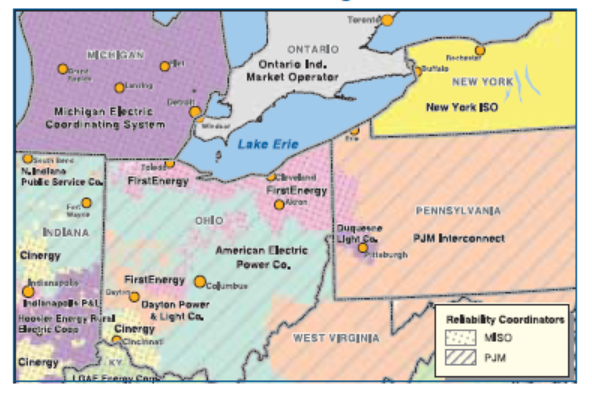
\includegraphics{rel_coord.png}
\end{center}
\caption{Reliability Coordinators and Control Areas in Ohio and Surrounding States}
\end{figure}

--10 regional councils, three effected on august 14th
East Central Area Reliability (ECAR), Mid-Atlantic Area Council (MAAC), Northeast Power Coordinating Council (NPCC)


5 RTOs/ISOs where affected
Midwest Independent System Operator (MSIO)
PJM Interconnection (PJM)
New York Independent System Operator (NYISO)
New England Independent System Opeartor (ISO-NE)
Ontario Independent Market Operator (IMO)

Initiating events of blackout involved two control areas
 - FirstEnergy (FE) and American Electric Power (AEP),
 and their respective reliability coordinator
- MISO and PJM


formation of



%%%
ch3 causes of blackout, failures to perform relative to policies, guidelines, standards of North American Electric Reliability Council (NERC) and, in some cases, deficiencies in the standards themselves.

QUOTE:  altough causes discussed produced the failures and events of August 14, they did not leap into being that day. Instead, as the following chapters explain, they reflect long standing institutional failures and weaknesses that need to be understood and corrected in order to maintain reliability

Four major causes of failures, seven violations of NERC standards

\begin{itemize}
\item Inadequte system understandin
FirstEnergy and ECAR failed to understand inadequacies of system, voltage instability and vulnerabiility of Cleveland-Akron area, and FE didnt operate system with approriate voltage criteria
\begin{itemize}
\item FE didn't conduct rigorous long-term planning studies, neglected multiple coningenciy or extreme condition analysis
\item FE did notconduct sufficient voltage analyssis
\item ECAR didnt conduct independent review or analysis of FE, allowing FE to use inadequate practices
\item Some of NERCS planning and operational requirments were ambiguous enough to allow this to happen
\item FE no under voltage load shedding program in Cleveland-Akron area
\end{itemize}
\item Inadequate situational awareness
\begin{itemize}
\item FE failed to ensure security by not using effective contingency analysis on routine basis
\item FE lacked procedure to ensure operation of critical monitoring tools
\item FE lack of internal communication procedures
\item FE lacked testing of monitoring tools
\item no backup monitoring tools to understand status of transmission system
\end{itemize}
\item Inadequate Tree trimming
- caused outages of three FE 345kV transmission lines, one 138 kV tranmsission line
\item Inadequate RC Diagnostic support
\begin{itemize}
\item MISO did not have real time information from a 345kV line (Dayton power and Light's Stuart-Atlanta) to become aware of the situationearlier
\item MISO was using non-real-time data to support real time monitoring, couldnt detect the N-1 seacurity violation
\item Lacked effective tool toidentify location and significance of breaker operation by emergency management system
\item PJM and MISO lacked joint procedure guildings on violation in other regions near borders
\end{itemize}
\end{itemize}

Violations from NERC policy
\begin{enumerate}
\item Following outage of Cham-Harding345 line, personnnel did not take necessary action to return system to safe operating state
\item Personnel did not communicate its emergency operating conditions to neighboring systems
\item FE state estimation and contingency analysis were not used to assess system conditions
\item MISO did not notify other reliability coordinators of potential system problems
\item MISO usingnot-real-time data in support of real-time operations
\item PJM and MISO lacked procedures between organizations regarding coordinations of actions to address security limit violation in others area near a common boundary
\item FE monitoring equipment not adequate to alert FE of important deviations from operating conditions
\end{enumerate}

FE 
did not demonstrate application of effective emergency operating procedures
did not demonstrate effective manual load shedding program to address voltage decays from uncontrolled failure of components

Lack of policy for
monitoring and cunctional testing of EMS and supervisory control and data acquisitioin systems and contingincy analysis
monitoring equipment not adequate, personnel not adequately trained to maintain reliable operation under emergency conditoins
require vegetation management program, but no management requirements
no specifics on coordinated procedures
no criteria for determining critical facility lists in area

ultimatily, complianciance is voluntary and decisions and standards are done through member votes.   standards are often administrative and technical rather than results oriented.  how much does nerc support these institutions to meet requirments.  policies or guidelines are inexact, lacking in detail. some regions have varied in willingness to implement exacting reliability standards. lack measurable compliance criteria


%%%
ch4 conditions on system, identificy contributions 

state of system in days and hours leading up to the event
at the time of first event (harding-chamberlin line trips), system was electrically secure and able to withstand occurrence of one of any more than 800 contingencies, including harding-chamberlintrip

however clear evidence that Cleveland-Akron area was highly vulerable to voltage instability problems, however it was still possible to operate system securely, however FE had not done long-term and operational planning studies to understand vulnerabilities and operational implications

NERC Definations
\begin{description}
\item[Reliability] The degree of performance of the elements of the bulk electric system that results in electricity being delivered to customers within accepted standards and in the amount desired.  Reliability may be measured by the frequency, duration, and magnitude of adverse effects on the electrical supply.
\item[Adequacy] The ability of the electric system to supply the aggregate electrical demand and energy requirments of the customers at all times, taking into account scheduled and reasonably expected unscheduled outages of system elements.
\item[Security]  The ability of the electric system to withstand suddden disturbances such as electric short circuits or unanticipated loss of systemelements.
\end{description}

geography, Cleveland-Akron area is a transmission constrained load pocket with relatively limited generation
at time of incident not at all time peak load

chapter discuesses system conditions in and around northeast Ohi
-electrical laods, real and reactive
- system topology
-generation availabiliity and capability
-power flows
-voltage profiles
-reactive power reserves


SITUATION

temperatures hot, but in normal range
Load in FE control area went up to 12,165 MW.  Operators had successfully managed higher demands before, all time peak was 13,299 MW.  Several large operators in midwest consistently under-forecasted load levels.  Forecasts are used for day-ahead planning and affect availability of equipment and schedules for following day.  High airconditioning loads is relevent because of low power factors (like other induction motors),  thus consuming reactive power.  persistant high temperatures strained areas limited reactive generation capabilities

generation units out of operation (not cause of blackout according to report, does not state whether it couldnt have prevented blackout though
-Davis-Besses Nuclear 883 MW, prolonged NRC ordered outage
Sammis Unit 3 180 MW forced outage 8/13
Eastlake Unit 4 238 MW, forced outage 8/13
Monrow Unit 1 817 MW planned outage on 8/8/03
Cook Nuclear unit 2, 1060MW, outageg began on 8/13

four or five capacitor banks within Cleveland-Akron area removed for routine inspectiion, including banks at Fox and Avon 138kV substations.important for voltage support, unable to return to service in afternoon despite need for more reactive power.
--Normal practice to do thisin off-peak season
--only First Energy knew of unavailability of critical resources, FE didn't recognize these as critical

3 notable unpanned outages occurred before 15:05 EDT
transmission lines on Cinergy 345,230,138kV system series outages and remained out throughout blackout, loss of lines not electrically significcant.  Cinergy made generation changes and  MISO implemented transmission loading relief (TLR) procedures

Stuart-Atlanta 346kV line, operated by DPL, monitored by PJM, tripped 14:02.  due to tree contact, remained out entire afternoon.  MISO did not know about status of line and lead to data mismatch that prevented MISO's state estimate producing usable results later

Eastlake Unit 5, 597 generating unit, major source of reactive power.  As operators tried to increase reactive power output, internal protection systems tripped the generator out of service.  Now needed to import 612 MW of power, making voltage management more challenging, loss of flexibility in operation

conditions at 15:05
Cleveland-Akron load = 6715 MW, 2402 MVAr
transmission losses = 189 MW, 2514 MVAr
reactive power from fixed shunt cacaitors = 2586 MVAr
reactive power from line charging = 739 MVAr
network config = after eastlake 5 outage, before loss of harding-chamberlin
area generation combined output = 3000 MW, 1200 MVAr

power flow into Cleveland-Akron area = 3900 MW, 400 MVAr
reactive reserves: 688 MVAr from generation in area
perry nuclear plant: 660 MVAr reserve capability

However 5\% drop in operating voltage, cause 10\% loss of shunt capacitor and line charging reactive power production (330 MVAr) and increases losses on lines (250MVAr)

Would be in precarious position with loss of Perry

inter-regional power transferws were high but within well established limits and previous experience.  these power flow transfers had limited effect on tranmission corridor containing Harding-Chamberlin Hanna-Juniper, and Star-South Canton 345 kV lines.

primarly increasing native load relative to limited amount of reactive power availableity caused deplation of reactive power reserves and thus declining voltages

critical corridor, four ciriuits
Harding-Chamberlin
Hanna-Juniper, Star-South Canton
Sammis Star
little through traffice, mostly serving native load in FE control area
no in area generation reserve
thus line loading not affected by events outside immediate vicinity, only cuts to load in Cleveland Akron area would be effective
redispatch of generation elsewhere would have little effect

however, the power flow patterns after the first trip on one of the 4 critical lines, would effect the ultimate path, location, and speed of the cascade after 16:05

on august 14, PJM implemented routine voltage management practies for heavy load conditions.  FE began requesting capcaittors to be restored and additional voltage support from generators
additional actions such as
plant redispatch and transformer tap changes 
voltages at Star Bus were at 98.5\% at 11:00 EDT and droped to 97.3\% after loss of Eastlake 5, 95.9\% after loss of Harding-Chamberlin
FE system operators reported this voltage typical for warm summer day, gradual decline in voltage with increase of load, normal considering no additional generation to provide reactive power support

NERCpolicy on voltages in generic terms, specifics done by each system.  FE's were minimum requirments, lower than and incompatible with its neighbors.  Good utility practice requires determination based on full set of V-Q (voltage performance realative to reactive power supply Q) and P-V ( real power transfer relative to voltage). for a wide range of systemm condition 13 billion in savings from ability to buy distant economical sources.

Precontingent voltage minimum of 90\%, versus mostly 95\% in surrounding areas, and not adequate for secure system operation.  FE predecssor Ohio Edison used 95\% to 105\% and 90\% post-contingency, which is compatible with neighbors.

reactive reserves fully depleted by 16:00 EDT in Cleveland Akron areas.  neighboring areas had sufficient reactive power and thus supported voltage levels, however needs to be injected at source, can't transport far.  Cleveland-Akron area had depressed voltages for days leading up to event, as well as hours leading up to event, and dropped below 95\% by 16:00 EDT

Voltage instability- can occur gradually within tens of seconds to minutes. imbalance of reactive power supply and demand, from iincreased real or reativeloads, high power transfers, loss of generation or transmission facilities.  Studied with V-Q and P-V analysis
V-Q evaluates reactive power needed to maintain voltage at a bus.  in stable conditions, as voltage increase, reactive requirments increase and as voltage drops, reactive reqs decrease.  however when the bus voltage decreases and reactive requirments increase, system is unstable.  The voltage at which this transition occurs is called critical voltage, and reactive power level at that point is reactive margin.  desired voltage should be well above this level.  circuit trips can cause critcal voltage to increase, reducing size of stable operating region and reducing size of reactive margin.
However, magnitude alone is poor indicator of voltage stability, V-Q analysis must be carried out for several critical bussess in local area covering range of load and gernatiion conditions and contingencies
P-V analysis determines power transfer capability acrrosss a transmission interface.  As power transfers reach a high level where stable voltage cannt be susustained, the point where last solved corresponds to critical voltage level.  This point is called nose.  System is stable before nose, and represents max power transfer.  contingency can lower the nose point

(other type of instability)
transient instability - generators swing out of synchronism with rest of system within a few seconds ofcritical fault

ultimately, nearby reactive reserves could not support Cleveland-Akron area.
no dynamic reserves, all static reserves, thus could not respond to changing conditions.  in addition, did not no critical voltages or max import capability.

VERY VULNERABLE

History of voltage instability
1994 June, 3 generators out, caused CEI to load shed (CEI is FE predecssor).  Used strict voltage criteria until 1998
2002 summer south canton 765kV to 345kV transorm, connects to FE Star line, experience overloadings, for 11 days. all actions short of load shedding used.  reduced life of transformer by 30\%.  AEP replaced this transformer.  AEP conducted extesive modeling to understand loss of transformer, reavealed that in combination with other outages, would cause significan low voltages and overloads.  AEP shared with FE. (jan 10, 2003)
studies showed that with high power transfer to north, expected overloading of transforming and depressed voltage if Perry unit and loss of Tidd-Canton Central 345kV line, and probable vascading into voltage collapse across northeast Ohio, for 9 different double contingencies.
AEP shared this with FE on May 21.  neither identify changes in transmission config or operatoring procedures which could be used during following summer to control pwower flow through S. Canton bank.

NONE of these voltage events or significant risks are reflected in any FE or ECAR seasonal or longer-term planning studiesor operating protocols.  FE's 2003 summer study was on N-1 events and no multiple contingency.  Only looked at thermal limits and voltages toremain within 90\% to 105\%.  assumed only missing david besse at peak load of 13,206 MW.  Real conditions were 12,166 MW, with 3 more generation outages, 180MW, 240MW, 597MW.  Study assumed all transmission in operation, despite outage of eastlake transformer and fo 1 capacitor, along with other capcaitors down.  Study used one set of import and export conditions, rather tahn a wider range of generation dispatch, import-export, andinter regional transfer conditions.  The study posited less stressful system conditions than really occured on Aug 14.

FE typically relied on ECAR to identify reactive power requirments, but ECAR did not do detailed analysis of Cleveland Akron area o in past 5 years, although considered operational considerstaion in 1990s and testimony filed in 1996 with FERC.  The voltage-constrained import was not studied and FE modified to less stringent voltage limits.  FE summer report identified potential overload of Star 345-138 transformers, but no mention of voltage limitation.

ECAR regional reliabliity council 1967
membership includes 29 major electricity suppliers serving 36 million people
budget 2003: \$5.15 million, including \$1.775 million paid to fund NERC.
AEP, biggest member pays 15\%, FE pays 8-10\%
18 full time employees, HQ Akron, Ohio
decisions dominated by member control areas, allow continuation of past practices instead of more stringent , consistent requirments for such things as voltage criteria and planning studies
PROBLEM: difficult for entity to declare members practices inadequate, when these members dominate the entity.  NERC is sufficiently vague and ambigous to allow this to happen as well.


Model-based analysis of the state of the REgional power system before the loss of FE's Harding-Chamberlin line
power flow of Eastern Interconnection
43,000 buses, 57,600 transmission lines, all major generating stations across northn US and eastern Canada
benchmarked by matching voltages and line flows to actual data at 1500 locations.  BASE CASE
ran contingency analysis on 800 possible events.  not resulted in violation of transmission line load or bus voltage limit, including Harding Chamberlin line outage.
Therefor, before, EI was operated within all established limits and full compliance of NERC's policies.  However, after Harding-Chamberlin trip, two contingencies would exceed emergency ratings immediately.

Perry first contingency, 1255 MW near lake Erie, critical to voltage stability of Cleveland Akron area.  Before 15:05, perry loss would lead to 93\% voltages and only 150 MW load margin (2\% of load).  However, after would have been close to voltage collapse.

FE had not planned for loss of Eastlake 5 and Perry, but should have been.  Loss of Perry has been recognized as single worst contingency for the area as far back as 1998., capacity of perry exceeeded total import capabilty of any 345kV circuit.  also no automatic load shedding procedures.

could not find FE contingency plan or operational procedure for loss of Perry.  V-Q analysis of loss of perry before and after event.
before - highest critical voltage at 90.5\%, way to close to acceptable voltages of 90\% to 105\% of normal operating procedures.  After, highest critical voltage is 92.5\%.

what would of happened with increased load?
tried 625MW increase
before loss of Perry, fine with voltages at 95\%,
after can only increase load 150MW before voltage instability

at 13:43 Perry plant notified control area of low voltages
at 15:36 askede about voltage spikes
at 15:42 still voltage spikes, close to tripping generator

System Frequencies
in stable conditions, frequency same across interconnectedgrid at any particular moment.  however depending on second-second balance betwween aggregate demand and aggregate generation the system frequency will vary.  This frequency is monitored on continuous basis.  No significant or unusual frequency ossicilation prior to 16:09 EDT.  not cause or precursor to initiation of blackout.  once cascade began, large frequency swings occured early and became principal means by which blackout spread across wide area.
on Aug 14th, frequency declines on order of 3200 MW per .1 Hertz or 1000 MW cause change of .031 Hz.

Time series studies indicate EI exhibis regular deviations, largest occuring in frequency that reflect changes at peak to off-peak schedule, and hourly and half-hour from changes such as ramp up and ramp down.  Frequency higher during early day with extra generation committeed and waiting to be dispatched at peak
frequency oscillation before 16:09 had no effect on blackout

System was in reliable state before 15:05.  While secure, still highly vulnerable, because some assumptions and limits were not accurate for safe operating criteria.  FE operating on very edge of NERC reliability standards.  vulnerability from lack of system planning and understanding

made worse by operators not adequetely trained or prerpared to recognize and deal with emergency situation  
IPP SIDENOTE:
independent power producers (IPP) began after passage of Public Utility rEgulatory Policy Act of 1978, established right of non-utility to operate and sell their energy to utilities.  1989 17.8\% of power purchased from other utilities and IPPs, 37.3\% in 2002
between 1986 and 2002, peak demand grew by 26\%, generation capacity by 22\% and little expansion in transmission capacity.
US DOE estimates \$13
IPP mostly don't get paid for reactive power productions.  sometimes contracts require to maintain voltage at buses which involves controlling reactive power outputs.  other times in emergency operators will dictate how much reactive power production they will need.  they will be paid in the difference of active power production they forgo by deviating from schedule.  it is requirement of operators not IPP to ensure reactive power requirments are there and make any short term arrangements to acquire these resources

%%%
ch5 conditions on the day, from bad situation to worse

How and why the blackout began

12:15 inaccurate input data rendered MISO's state estimator ineffective
13:31 FE Eastlake 5 generator tripped
14:14 alarm and logging in FE control reoom failed and not restored until after blackout
15:05 FE 345kV lines start tripping due to contact overgrown trees within lines right of way areas
15:46 FE, MISO, neighbor utilities realize FE system in jeoardy, possibly able to avert crisis by droppping at least 1500MW of load around Cleveland Akron - no effort was made
-after loss of key 345kV lines, underlying network of 138kV began to fail, leading to
16:06 FE losses Simmis-Star line -- triggered uncontrollable 345 kV cascade 
even after most of akron area blacked out, most of norther Ohio still interconnected and had heavy load.  Loss of overburdened sammis star line instantly overloaded lines in adjacent areas and cascade spread rapidly by protective relay action to avoid physical damage

Phase 1 - normal to bad morning

load moderately high, air conditioning demand consuming large amounts of reactive power
2 key generators down (Davis-Besse and Eastlake 4) for both active and reactive load
Loss of Eastlake 5 depleted critical voltage support.  Did not directly cause blackout, but made transmission line loadings higher than normal, altough still within normal ratings

14:02 DPL Stuart-Atlanta 345kV line tripped due to tree contact 
-- did not effect FE system, but rendered MISO's state estimator ineffective between 12:15 and 15:34  MISO unable to perform contingency analysis - could not determine that without Eastlake 5, system no longer N-1 stable, for instance if FE lost major transmission line

Peak load conditions on less than peak load day, voltages low but consistant with hostorical voltages.  FE reliability operator concerned about low voltage as early as 13:13.  Asked for voltage support, no generators were asked to reduce real power output to produce reactive power.  Tried to get shunt capacityors at Avon restored, but unable to.

After loss of Eastlake 5 at 13:31 voltage concern increased
13:43 asked plants for more voltage support

MISOs state estimator - usual run every 5 minutes, Real Time Contingency analysis (RTCA) less frequently
12:15 SE produced solution with high mismatch from real conditions
(traced to outage of Cinergy's Bloomington-Denois Creek 230 kV line, not updated in MISO's SE)
Suppose to be done through ECAR data netowrk, but link for that line status had not been established.
13:00 problem fixed and SE produced good solution and followed with RTCA.  However automatic 5 minute trigger on SE turned off and not re-enabled.  Thinking system restored, analyst went to lunch
14:40 SE 5 minute re-enabled but failed to produce solution (due to Stuart-Atlanta line at 14:02)
--discrepency between MISO and real world
MSIO tried to solve with Stuart-Atlant line in service until 15:29
called PJM to verify, 
15:41 finally solved and ran successful RTCA.
16:04 back to full automatic operations
%%%
EMS and decision support tools
Contingency analysis driven from state estimation using data fed from SCADA system
System Control and Data Acquisition (SCADA)
Three types of elements (RTU, communication betwixt, master stations)
field remote terminal units (RTUS) - gather info such as status of breaker, voltage, real and reactive power can execute control operations such as opening or closing a breaker, can communicate with SCADA Master Stations, or sometimes other RTUs
Master station - initiate data gathering cycle, few seconds to several minutes.  integrating into control room, direct interface to Energy Management System (EMS), recieve data from field RTU and relay control operation to field devices for execution
State Estimation - use real time data from subset of facilities to find configuration of whole network
Contingency analysis - given state estimators representation of system, analysis impact of specific outages, or higher load, generation changes, effects on security.  Try to identify overloaded lines or voltage violations if event occurs.  Many areas do not do real time contingency analysis, others run after significant system events
%%%

Cleveland Akron typically supported by generation of Davis-Besse Perry and Eastlake, and significant imports with alot from 9100 MW of generation on Ohio, Pennsylvia Border
Trip of Eastlake 5
FE load of 12:080 MW, import 2575 MW 21\%, FE need for reactive power rose.
loss of Eastlake 5 caused system to be N-1 unstable after loss of Harding-Chamberlin line
FE did not perform contingency analysis after loss of Eastlake 5, nor after loss of Harding-Chamberlin.  Did not discover that system was no longer N-1 secure at 15:05 and needed operator action

Line trip of Stuart-Atlanta only important due to rendering MISO's SE ineffective

%%Data Exchange
topology and impedence modeled in power flow programs, SE, and contingency analysis to evaluate and manage system
ICCP Inter-Control Center Communication NERCNet opearted by NERC, used for minute to minute operation, such as line flow, voltage, generation levels, interchange schedules, area control eroor ACE, system frequency
IDC - Interchange Distribution Calculator, determine where power will actually flow, 40,000 buses, 55,000 lines, 6,000 generator model TDFs, transfer distrubtion factor for power transfer and OTDF outage transfer distrubtion factor, 
SDX - element status information, some update once day while others after event occurs, no regulation at time of writing
Etags - vital accessory information
Voice communication


Phase 2 - FE computer failures

14L14 FE control room lost alarm function, next lost remote control consoles and then primary server by 14:54.  For over hour no one knew computer system not operating properly, even though IT knew and were working to fix.  FE operators unaware of degrading system.  Used outadated system info to discredit information from others on growing problems

The failure of system is significant but just as significant is that operators didn't know system failed.  Operators surprised by calls from MSIO, AEP, PJM, FE field operation which provided conflicting info on system.  Alarm system had stalled in processing and did not process anything after this event.  This buildup of events overflowed input buffers and took down server

14:20 FE remote consoles failed, IT auto-paged
14:27 Star South Canton 245kV tripped and reclosed
14:32 AEP notified FE, FE had no log of this
14:41 primary FE control system server failed, passed to backup - IT auto-paged
14:54 FE backup computer failed, IT auto-paged
IT did not notify control room
server failures led to screen updates as long as 59 seconds per screen, versus typical 1-3 seconds
15:08 warm reboot successfail.  however alarm system still failed and IT did not confirm if it was working properaly after reboot
AGC not working during server downtime (automatic generator control to allow gernators to respond to load in real time)
14:54 to 15:08 and 15:46 to 15:59
Loss of servers flatlined reliability charts such as raw Area Control Error (ACE), FE system load, Sammis=Sout Canton and Sout Canton - Star loadings.  Loss of ACE was not bad.
15:33 AEP identified overloads on a Sammis-Star line loss and asked PJM for corrective action plan, but not done before line tripped out.  AEP called FE 3 times between 14:35 to 15:45 to find out if FE knew cause of outage
FE had problems with alarm processing prior, but could not find cause of this behavior.  Determined only way to fix would be cold reboot.  Disccussed possibility at 15:42, but decided system to precarious to do., lose even more function for extended period of time.

FE control room becoming aware,
hint 1 at 14:19 when caller said 3 center dial=ups had failed
14:25 caller said failure of 3 remote consoles
14:32 scheduling changes, but totals were not updaing

IT first notified of alarm issue at 15:42.  IT never notified of server problems before or after fix at 14:54.
RESORT to telephone and direct analog telemetry
lots of calls with relevant information, but operators did not recognize emerging problems.  including eastern control center, perry nuclear plant asking about line trippings.  AEP line trippings, MISO PJM about possible line overloads
without alarms, FE operators ignored pertintent info as not effectivng system


Phase 3 - FE loses three 345kV lines

between 15:05 and 15:41 three lines trip, flows at or below emergency rating, each result of contact with line and tree
as elments tripped, flows shifted and voltages on FE systems degraded

15:05 Harding-Chamberlin 345 line tripped
15:31-33 MISO call PJM to determine status on Stuart-Atlanta line. PJM - line was out
15:32 Hanna-Juniper 345 line tripped 
15:35 AEP asked PJM to work on 350 MW TLR to relieve overloading on Star-South Canton, not knowing of Hanna-Juniper trip
15:36 MISO call FE regarding post-contingency overload on Star-Juniper 345, for contingency loss of Hanna-Juniper trip, unaware this had already happened
15:41 Star-South Canton tripped, reclosed, tripped again

Harding-Chamberlin tripped due to contact with conductor and tree at about 44\% of normal (emergency) line rating.  Escalated by loss of Harding-Chamberlin, Hanna-Juniper line failed at 88\% of normal line (emergency)  rating due to contact with tree.  Star-South Canton made three serpate contact with tree finally going out at 93\% of its emergency rating.  Failure not due to overloading or high conductor temp, but because hit an overgrown, untrimmed tree
no prior sustained outages due to tree-line contact in 2001,2002,2003.  Flyovers said problems in 2001,2002, but not in 2003, flyovers not effective enough, need ground patrols.

Line ratings set to keep internal temperature below level, such as 90 degrees for normal and 100 degrees for emergency, allowed for a short period of time.  Most of FE ratings limited by capabilities of terminal equipment rathor than conductors.  Calculating summer ratings, FE used 32 degree C for ambient temportures and 1.2 m/sec for wind speed, which is relatively high and would be favorable.  Temperature was 31 degrees on day, however wind speed was between 0 and .6 m/sec

Easements for transmission rights-of-way include
right to erect, inspect, operate, replace, relocate, repair, patrol, permanently maintain upon,over,under, and along the above described right of way across said premises all necessary structure,wires, cables, and other usual fixtures and appurtenances used for or in connection with the transmission and distribution of electric current, including telephone and telegraph, and the right to trim, cut, remove, or control by an other means at any and all times such trees, limbs, and underbrush within or adjacent to said right of way as may interfere with or endanger said structures wires or appurtenances or their operation

FE used 5 year cycle, consistent with industry practices.  NERC has no standards or requirments for vegetation management.  common industry practices need significant improvement to ensure greater reliability
tree growth during spring and summer, later in summer is more vulnerable due to growth.  as temp increases, AC load increases, high load heats up line and hot lines sag.  most emergency ratings attempt to limit conductor temp to 100 degrees C. wind flow increases cooling effect, wind speed was low in area.

After Harding-Chamberlin and Hanna-Juniper trip, 1200 MVA power flow needed to find new path to reach load in Cleveland.  This increased loading on remaining 345kV lines and pushed more power onto 138kV system.
due to loss of SE and RTCA, MISO did not recognize Hanna-Juniper loss, and FE did not know of its loss or consequences.
to relieve problems, use Transmission loading relief (TLR) measures. prevent system from operating in unreliable state.  Neither AEP nor PJM realized Hanna-Juniper line tripped. Also TLR request for 350 MW is high, operators wanted confirmation of why so much reliefe needed.  Unfortunately, most loading was due to native load, so only effective measure would be load shedding by FE in Cleveland.

Loss of Star-South canton due to multiple tree contacts from 14:27  (less than 55\% capacity) to final one at 15:41 (93\% capacity).  loss of line increased flows on 138 kvsystem and only remaining 345 kv line, Sammis start.  voltages degraded in cleveland on 138kV and 69kV system.  Load shedding of 500Mw to 1000MW would have increased voltage at star bus and reduce line loading from 91\% to 87\% perhaps stopping ultimate lockout of Sammis-Star line

Impacts from 345kV failures.  (good picture of effect on Sammis-Star line loading)

15:42 FE operator informed IT that EMS system functionality compromised, nothing is updating, we are recieving calls reporting trips but nothing in event summry, something wrong.  first evidence of FE control room recognize degradation of EMS system.  
15:42 Perry plant called, lots of voltage spikes, not sure how much longer can survive.
15:46 Perry called, not looking good, not going to be here much longer, then you have bigger problems.
15:48 PJM called MISO to report Star-South Canton trip, but line flows didn't match on Sammis-Star
15:56 FE informed PJM that Hanna-Juniper also out, FE believe problems outside of their system 

Emergency Action
Utilities have plans to reduce load, calling customer load reduction, public appeals, voltage reductions, finally load shedding system, cutting off interruptible and firm customers, FE plan updated yearly.  However, even in emergency conditions ( it was recognized AEP PJM in discussion of tripping 138kV lines no practical way to mitigate overloads across utilities and reliability coordinator boundaries.
FE ramined unaware of precarious conditionsm grasped trouble at 15:45, but never decalred official emergency condition.
part of problem internal communcations, operators did not inform other operators of critical clues.
-physical seperation of operators, voltage and transmission seperator
-lack of shared log
-systematic procedures at shift change
-infrequent trainging in emergency situation
FE has written procedures but did not follow because unaware system needed

no training for major disturbance or emergencies, no training consideration for emergency operation


Phase 4 - collapse of 138 and loss of Sammis star

15:39 first of 16 138kV lines trip
15:39-15:58 - seven lines had tripped
15:59 5 lines tripped due to breaker failure at West akron bus
16:00 - 16:08 4 138 lines tripped
as 138kV lines tripped, voltage sensitive customers dropped, dropping 600 MW of load

16:05 - Sammis Star line tripped
unlike contact to tree, tripped by apparent low voltage due to protective relay, low impedence from depressed voltage divided by abnormally high line current.  acted as if short circuit. 
THIS marked turning point of system which initiated a cascade blackout across northeast US and Ontario

Amount of load shedding needed to fix problem grew rapidly as conditions deterioarted.
Before Sammis star outage, 1500MW load shed may have prevented cascade.

FE had no automatic load shedding and did not attempt manual load shedding.  Within 6 minutes of these overloads and extremely low voltages, big power swings and accelerated line tripping would cause sepeartion and blackout within the Eastern Interconnection

%%%
ch6 cascade portion as it spread

blackout rare, variable
initiating events vary, human actions, system topology, load/generation balace
power transfers, voltage profiles, protective relays
some start with multiple line trippings
natural / common causes, wind lightning, heat
fault causes high current, low voltage on line of fault
protective relay detects high current, low voltage, trips to isolate from system

dynamic phenomenon
sequential tripping of transmission lines and generators in a widening geographic area
power swings and voltage fluctuations cause other lines to detect high current low voltage, even if faults do not exist
generators tripped off to protect from power voltage swings
protective relay work well to protect individual
but harmful to whole, propogating blackout spread

Impedence Relay
$Z = V / I$ 
$Z$ apparent impedence,
$I$ current
$V$ voltage

zone one faults $80$\% of line next to relay, no time delay
zone two, entire line and slightly beyond, slight time delay
zone three, slower acting, faults well beyond line length
protect lines from faults and may trip from apparent faults by large swings in voltage and currents


Series line outages at 15:05
heavy loading on parallel circuits 
FE Sammis-Star 345 line tripped 16:05
triggered cascade of interruptions on high voltage network
electrical fluctuations and facility trips
within seven minutes blackout rippled from Cleveland-Akron across much of northeast United States and Canada

by 16:13
508 generating units at 265 power plants
tens of millions people without power

\begin{figure}
\begin{center}
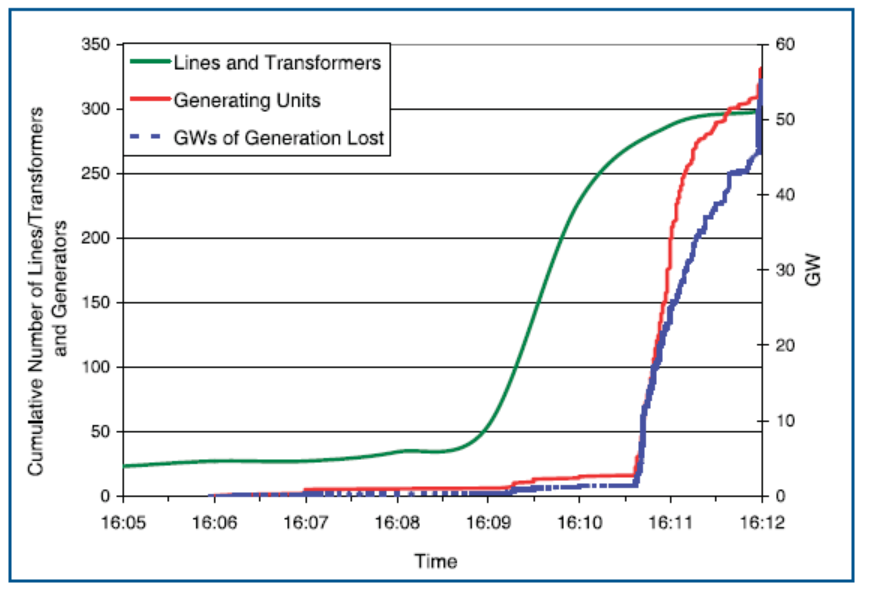
\includegraphics[scale=.57]{line_outage_over_cascade.png}
\end{center}
\caption{Rate of Line and Generator Trips During the Cascade}
\end{figure}


Started relatively slowly
then stopped in 3 minutes

Phase 5
Collapse of FE's transmission, unplanned power shifts across region
electricty flows moving generators in south and west to load centers in ohio, michigan, ontario
series of lines tripped in northern ohio high loads, hastened by zone three operations
shift in power flow and loadings, but grid stabilized after each

Phase 6
after 16:10:36
power surges from FE system failures neighbors saw overloads and impedence relay operated
wave of line trips through wester Ohio, seperated AEP from FE
line trips up into Michigan, seperating east and west, power flow reversal within michigan towards cleveland
zone 3 relay actions acceleratied line trips, reducing operator time to react

paths cut from west
power surge from PJM into New Tork and Ontario
in counterclockwise direction around lake
to serve load in eastern Michigan and northern Ohio
Relays between PJM and New York saw this surge as fault and tripped lines
Ontario east west overloaded and tripped
northeastern United States and eastern Ontario electrical island
large area importing power before cascade, unstable after 16:10:38
once northeast split from rest of EI, cascade was isolated

Phase 7 
after 16:10:46
large island had less generation than load, unstable
large power surges swings in frequency and voltage
many lines and generators tripped
breaking into several islands
the imbalance between generation and load in island unbalanced, further trippings until
equilibrium established in each island
some islands survived, such as one supported by
large Beck and Saunders plants in Ontario and
765kV interconnection to Quebec
others collapsed into blackout



\begin{center}
\includegraphics[scale=.75]{cascade_page.pdf}
\end{center}


Why stop?

effects of disturbance as travel become damped
voltage and current swings from afar not as sever
high voltage more densely networked lines better able to absorb voltage and current swings
--barrier to spread of cascade

line trips isolated portions
many retain sufficient online generation
was sufficient gernation to match load and stabilize situation (voltage and frequency)
coupled with fast-acting automatic loading shedding

Sammis-Star tripp 16:05:57, zone 3 relay action
no longer differentiate between three-phase fault and exceptionally high line-load
reactive flow VAr ten times higher than earlier in day

four of five 48 MW turbines tripped off, under voltage 16:07
overloading and tripping within Ohio slow enough system readjust and find stable condition
East Lima-Fostoria at 16:09:06
cut main energy path from south and west into Cleveland and Toledo
flow from MECS to FE jump from 200 to 2300

\begin{figure}
        \centering
        \begin{subfigure}[b]{0.5\textwidth}
                \centering
                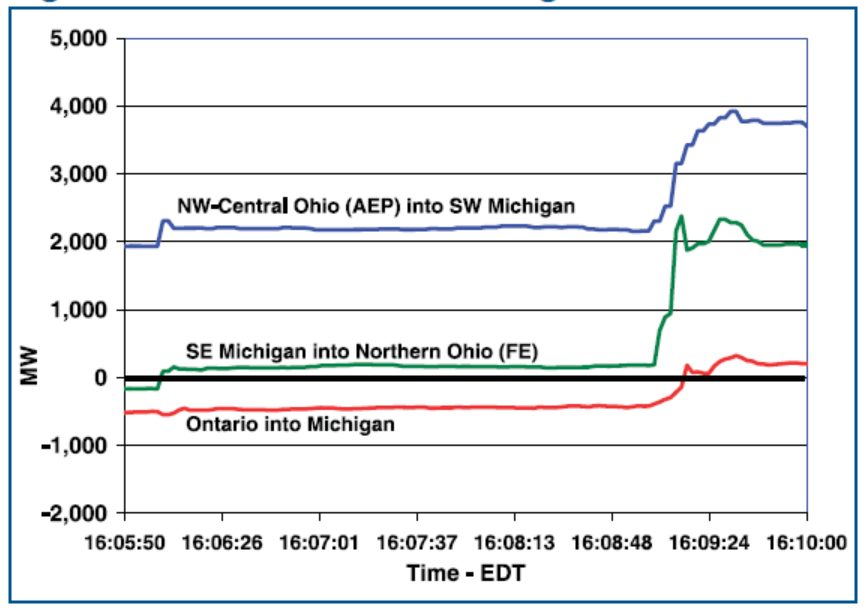
\includegraphics[width=\textwidth,height=2in]{line_flows_into_michigan.png}
                \caption{Line Flows into Michigan}
                \label{fig:gull}
        \end{subfigure}%
        ~ %add desired spacing between images, e. g. ~, \quad, \qquad etc.
          %(or a blank line to force the subfigure onto a new line)
        \begin{subfigure}[b]{0.5\textwidth}
                \centering
                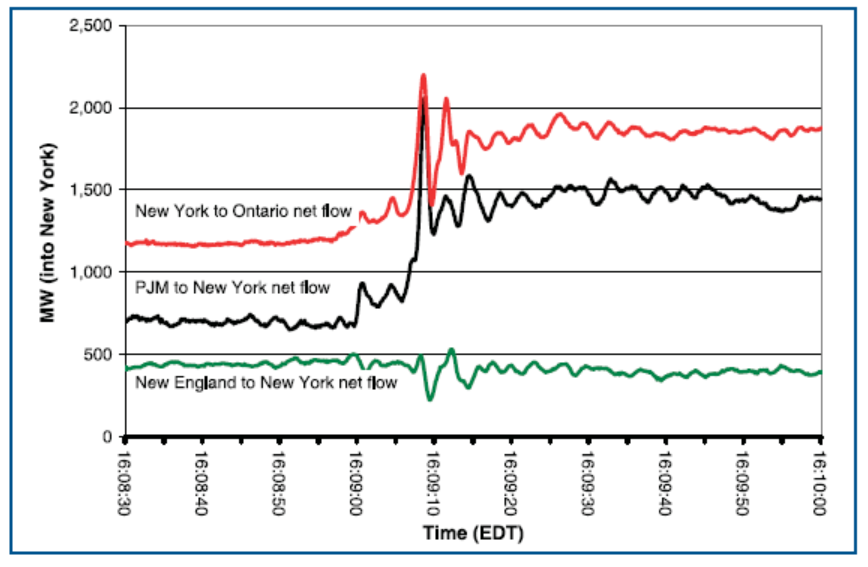
\includegraphics[width=\textwidth,height=2in]{line_flows_into_newyork.png}
                \caption{Line Flows into New York}
                \label{fig:tiger}
        \end{subfigure}

        \begin{subfigure}[b]{0.485\textwidth}
                \centering
                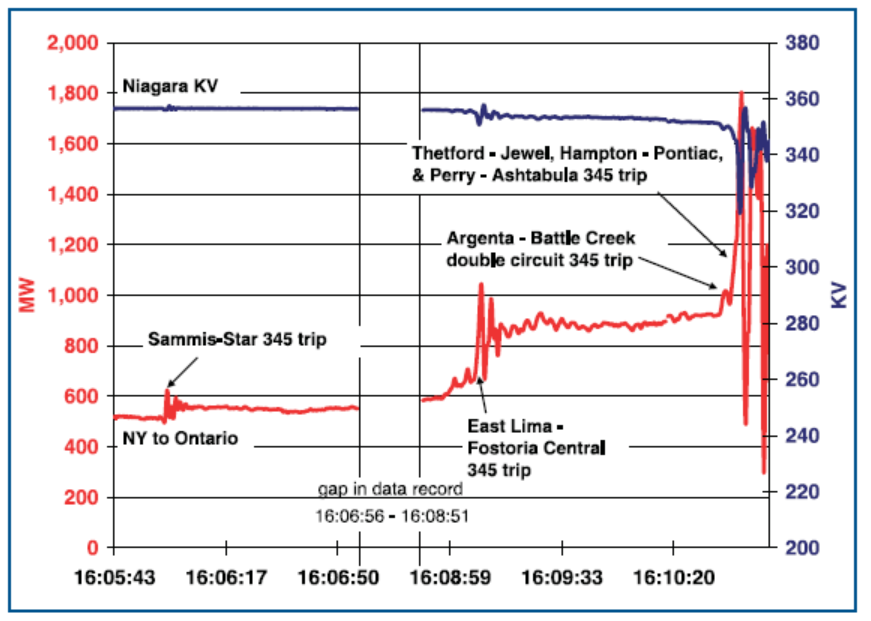
\includegraphics[width=\textwidth,height=2in]{line_flows_newyork_ontario.png}
                \caption{New York to Ontario}
                \label{fig:tiger}
        \end{subfigure}
        ~ %add desired spacing between images, e. g. ~, \quad, \qquad etc.
          %(or a blank line to force the subfigure onto a new line)
        \begin{subfigure}[b]{0.485\textwidth}
                \centering
                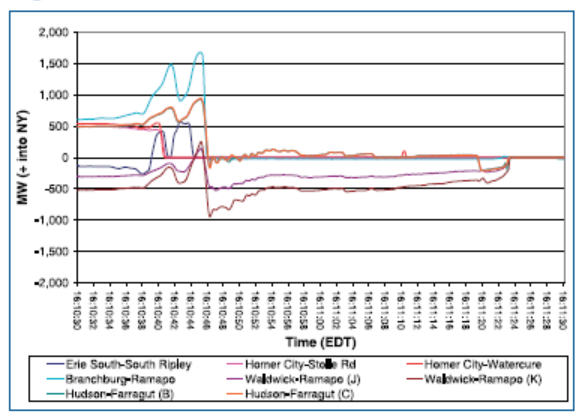
\includegraphics[width=\textwidth,height=2in]{line_flows_pjm_newyork.png}
                \caption{PJM to New York}
                \label{fig:tiger}
        \end{subfigure}
        \caption{Line Flows in Cascade}\label{fig:animals}
\end{figure}

16:08:59 Galion-Ohio Central-Muskingum 345kV line trip
16:09:06 East Lima-Fostoria Central 345kV line trip
-automatic load shed programs may have saved at this point
- large power swing from Pennsylvania and New York through Ontario to Michigan

low voltages in Cleveland area made difficult to maintain synchronism with EI

if lines not tripped on zone 2, 3
might have gotten heavily loaded lines and 20-30 minutes before line sag into something and ground fault
Dale-West Canton line took 20 minutes to trip under 160-180\%
unable to determine length of time
but would have period to readjust and taken action by load shedding

16:09:08 to 16:10:27 power plants tripping

16:10:36 to 16:13 thousands of events occurred on grid, when over much in dark

16:10:36-16:10:39 lines tripp michigan, norther ohio, lost generation, northern ohio seperate from pennsylvania

16:10:38 power flow surge after loss of paths in michigan and ohio
surge lowered voltages and increased currents on lines along Pennsylvania-New York

large magnitude so frequency not the same across EI
plummeting voltages in Detroit and loss additional local generation, lose synchronism and black out 16:10:43

\begin{figure}
\centering
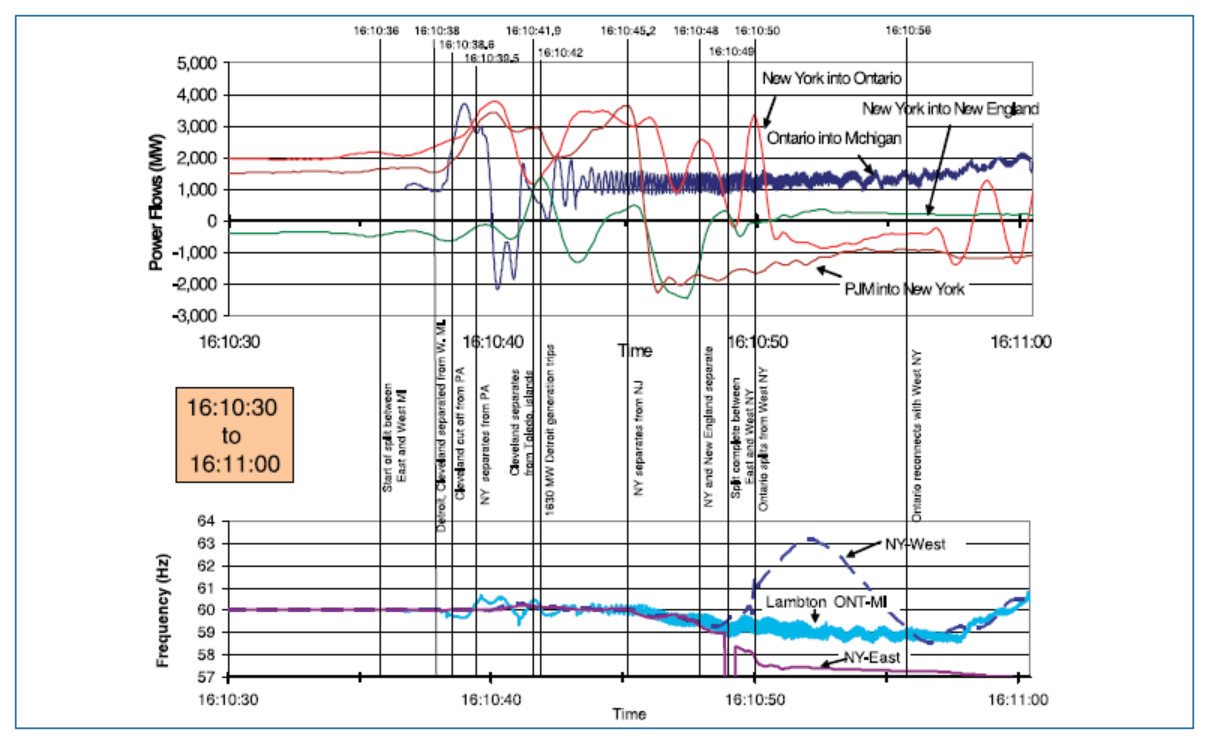
\includegraphics[scale=.75]{key_events.png}
\caption{Key Events During Cascade}
\end{figure}

series of circuits trip between PJM and NYISO due to zone 1, overload and depressed voltage
-large power swings between other areas where overloading there circuits

16:10:39 to 16:10:46
345kV line trips in ohio michigan 
load shedding FE shed 1750 MVA load, AEP shed 133 MVA load
seven power plants tripp, 3294 MW in Ohio
four power plants trip, 1759 MW Detroit

caused power flow change of 5,800 MW, 3,700 MW westbound to 2,100 eastbound across Ontario to Michigan

16:10:39-16:10:44 Western Pennsylvania seperate from New York
16:10:43 to 16:10:45 disconnected in New Jersey and northern Ontario, isolating northeast portion of interconnect


seperation of New York, Ontario, and New Englend from rest of Eastern Interconnect

to south and west, remaining EI at 60.3 Hz, excess 3,700 MW generation disconnected from load it was serving


Phase 7
Electrical Islands form in northeast US and Canada
16:10:46 to 16:12
16:10:46 New York New England disconnected
16:10:50 Ontario from New York
16:11:22 Connecticut from New York
16:11:57 Ontario from Michigan


QUOTE: As the cascade progressed beyond Ohio, it spread due not to insufficient reactive power and a volt- age collapse, but because of dynamic power swings and the resulting system instability. Figure 6.7 shows voltage levels recorded at the Niagara area. It shows clearly that voltage levels remained stable until 16:10:30 EDT, despite sig- nificant power fluctuations. In the cascade that followed, the voltage instability was a companion to, not a driver of, the angle instability that tripped generators and lines


that is good argument for using DC model, the angle instability tripped generators and lines, while voltage was an amplifying parameter

also, i believe the size of the ripples through the system are proportional to the amount of imbalance in net injects between neighboring clusters



Why the blackout stop?
designed such that threatened equipment disconnect from system
generators most expensive, disconnected as self-protective measure
then in good condition to rebuild system once blackou over

race between relay and power surges
longer lines tripped first,
relay settings with longer apparent impedence

midwest had voltage problems and no reactive reseres
pjm new york new england anticipating high demand, had more reactive reserve online


automatic load shedding

under-voltage
89 - 92\%
eliminate load to restore reactive power relative to demand, 
contain voltage problem

under-frequency (UFLS)
stablize generation load after electrical island form
reflect how well load and gen balanced
NERC requirment shed at least 25-30\% of load within each region
load progressively dropped based on frequency

UFLS
1883 MVA Ohio
Michigan 2835 MW
New York 10,648 MW in numerous stteps
PJM 1324 MVA
Ontario 7800 MW 2 steps
New England 1098 MW

even if it worked, oscilations made stabilization difficult and unlikely

Generator trips
Quebec 5 plants
Ontario 92 plants
New England 31
MISO 32
New York 70 
PJM 35

Convential steam 66
Combustion 70
Nuclear 10
Hydro 101
Other 18

6\% tripped at start 16:05:57 - 16:1038

10\% when Michigan New York Ontario New England seperate from EI
84\% tripped after island formed, with frequency change my 3 hz, 100 times normal deviation


loss of generators before island bad
protection points shut down unit to early, to make balance harder

some voltage tripp at 90\%, but stall point for motor is 70\%, why is this so
some trip off from using grid power, not quality enough for in house auxillary equipment


\begin{figure}
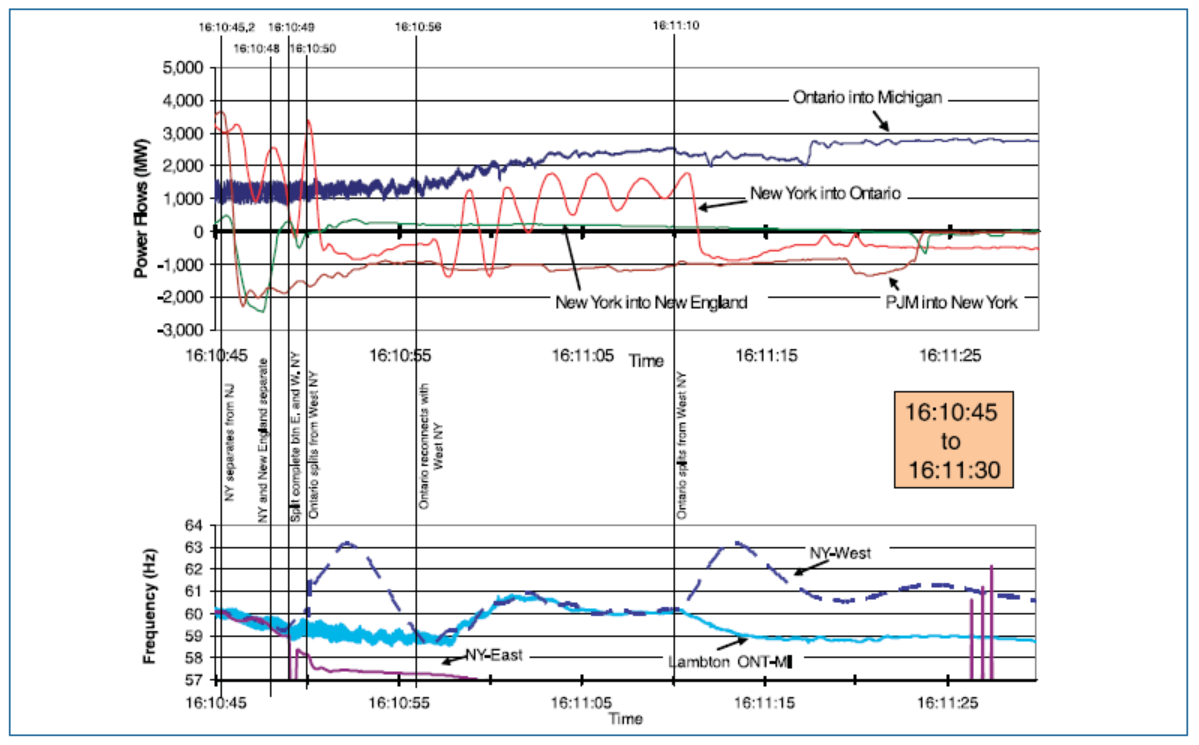
\includegraphics[scale=.75]{key_events_2.png}
\caption{Key Events}
\end{figure}

New York - New England disconnect 16:10:46 to 16:10:54
generation deficiency in Michigan and Ohio
New York split East - West 16:10:49
frequency down to 58 Hz, 7115 MW UFLS

inherent weak points
tend to be points with highest impedenance, long overhead lines with high loadings

even after 40\% load shed, dynamic conditions on grid
frequency falling, flows and voltages oscillating, power plants tripping
slow islanding and more generation might have made balance possible


One large island remained in opeartion, serving 5700 MW demand, western New York
Niagara and St. Lawrence hydro plants

basis for restoration in New York and Ontario

%%%
ch7 comparison with previous outages

short local outages fairly frequent
system wide disturbance rare, occur more frequently than normal distrubtion
electric power systems fairly robust, capable of withstanding one to two contingencency, but fragile with respect to multiple contingency events, unless readjusted
shrinking margin in current transmission syste,
likely to be more vulnerable to cascading outages, than in past
absense of transmission projects with significant voltage
system harder to run reliably
opearted closer to edge of relability

compare
\begin{itemize}
\item Northeast blackout Nov, 9 1965
\item New York City blackout July 13th, 1977
\item West Coast blackout Dec 22, 1982
\item West Coast blackout, July 2-3, 1996
\item West Coast blackout August 10, 1996
\item Ontario and US North Central June 25, 1998
\item Northeast outages and non-outage disturbances, summer 1999
\end{itemize}

November 9, 1965: Northeast blackout
20,000 MW load, 30 million people
All New York, Connecticut, Massachusetts, Rhode Island, small segments north Pennsylvania, northeastern New Jersey, Ontario
lasted up to 13 hours
formation of North American Electric Reliability Council 1968

backup protective relay operated, opened 1 of 5 230kv power lines.  when flows redistrubted, remaining 4 tripped within 2.5 seconds.  resulting power swings cascaded Northeast
-protective relay take line out at 375 MW setting
-operating personnel not aware of set point
-230kV line out by overcurrent relay action, several 115 230 out by protective relay action
-two key 345kV lines due to instability 
-lower voltage lines tripped open
-5 of 16 generators tripped from predetermined operating procedures
- 10 generating units at Beck shut down low governor oil pressure, 5 pumping generators off by overspeed governor control
-other lines on under-frequency

July 13, 1977: New York City

6000 MW, 9 million people
up to 26 hours
series of events seperated Consolidated Edison from neighboring system
collapse began 2 345kV lines on common tower struck by lightniing atnd tripped
-caused electrical sepeartion then collapsed.  
Generation within enough sufficient to serve load, with loss of imports
circuit breaker operation isolated Indian Point 3, dropping 883 MW load.  loss of ring buss 345kV tie, importing 427 MW
total loss of 1310 MW
18 minutes, 2 more 345 drop to lightning strike, only one recconencts
isolated Consildated Edison
resulting power surge caused line trip
23 minutes later line trips due to sagging into tree
345kV to 138kv transformer overloaded
7 minutes later tap-changing mechanism failed on phase shifter, loss of 1150 MW imports
remaining 138kV ties to interconnect overload and trip
insufficient generation in isolated system, lead to collapse

December 22, 1982: West Coast Blackout

12,350 MW load loss, 5 million people
high winds take down 500kV line tower, into parallel 500 kv line tower, both lines lost
fell into two 230kV lines underneath, collapsing 230kV lines
remedial action scheme to seperate interconnect into two islands, and trip generation in one to minimize customre outages and recovery
delayed operation of scheme, seperated into 4 islands
-problems with coordination of protective schemes, operated slowly or not at all
poor communication channels
backup schemes failed because coordination of relay settings not anticipated for this server disturbance
non-uniform data and time formats

July 2-3 1996: West Coast Blackout

28000 MW load, 7.5 million people
Arizona, California, Colorado, Idaho, Montana, Nebraska, Nevada, New Mexico, Oregon, South Dakota, Texas, Utah,  Washington, Wyoming, Alberta, British Columbia, Baja California Norte
upto 9 hours
loss of major transmission lines and generation from McNary Dam, seperated into four islands
Heavy north-south power transfers, southwest demand by hot weather and excellent hydroelectric conditions in Northwest and Canada
High temps in Northwest caused lightly loaded transmission to sag into untrimmed trees and trip, third heavily loaded line trips from tree
led to overload and outage of additional transmission
loss of McNary due to incoorrectly applied relays
power oscillations on California to Oregon intertie trip from protective relay
seperate western interconnect into four grids

operators not aware system unsecure for hour after first two lines outage, no new oeperating studies been performed

June 25, 1998: Upper Midwest Blackout
950 MW load 152,000 people
Minnesota, Montana, North Dakota, South Dakota, Wisconsin, Ontario, Saskatchewan
19 hours
lightning storm initiated series of events causing system disturbance
345 line struck by lightning and tripped, lower voltages overload and trip
seceond 345 line taken out by lightning
remaining lower voltage overloaded and tripped out by protective relay

Summer 1999: Northeast US Non-outage disturbance
PJM load 51,600 MW, 5000 MW above forecasted, used emergency procedures beside tripping load to serve record customer demand
steep voltage declines due to high transfers across system
reactive supply inadequeate, shunt capacitors out of service


Comparison

common factors
\begin{itemize}
\item conductor contact with trees, initiating trigger many times, loss of more than one circuit, multiple contingency, happens during high inductive load (air conditioning, irrigaation) along with hot weather, heavy burden on lines.  losing circuits contributes to voltage decline, drawing additional reactive power supply
\item over-estimation of dynamic reactive output of system generators, factor in most of events, made by shunt capacitors and generating resources, in most events assumed reactive output of generators greater than generators actually produced. limited by over-excitation limits or derated due to high ambient temperatures. other generators in fixed power factor and did not supply more reactive power in depressed voltage conditions
\item inability of system operators or coordinators to visualize events on entire system, only can see within territory, however these events go across territories, need to see neighbor as well, better communication and displays
\item failure to ensure system operation within safe limits, operators unaware the vulnerability of system, inaccurate modeling, no visibility, no monitoring of stability, no reassessment after significant event
\item lack of coordination on system protection - coordination of system protection, system wide controls to protect interconnection rather than individual piecies
\item ineffective communication
\item lack of safety nets, such as load shedding programs, almost always can make from having worse situation
\item inadequate training, training in distrubance simulation
\end{itemize}


Changing conditions that affect system reliability
\begin{center}
\begin{table}
\begin{tabular}{| p{7cm} | p{7cm} |}
\hline
Previous Conditions 	&	Emerging Conditions 		\\	\hline  	\hline
Fewer, relatively large resources	&	Smaller, more numerous resources		\\	\hline
Long-term, firm constracts 	&	Contracts shorter in duration, more non-firm transactions, fewer long-term firm transactions	\\	\hline
Bulk power transactions relatively stable and predictable	&	Bulk power transactions relatively variable and less predictable	\\	\hline
Assessment of system reliability made from stable base (narrower, more predictable range of potential operating states)	&	Assessment of system reliability made from variable base (wider, less predicatable range of potential opearting states)		\\		\hline
Limited and knowledgable set of utility players 	&	More players making more transactions, some with less interconnected operation experience; increasing with retail access	\\	\hline
Unusued transmission capacity and high security margins	&	High transmission utilization and operation closer to security limits	\\	\hline
Limited competition, little incentive for reducing reliability investments	&	Utiliities less willing to make investments in transmission reliability that do not increase revenues	\\	\hline
Market rules and reliability rules developed together	&	Market rules undergoing transition, reliability rules developed seperately	\\	\hline
Limited wheeling	&	More system throughput	\\	\hline
\end{tabular}
\caption{Changing system conditions}
\end{table}
\end{center}
%%%
ch 8 nuclear plant performance

%%%
ch9 security, cyber security

%%%
ch10 recommendations



%%%%%%%%%%%%%%%%%%%%%%%%%%%%%%%%%%
